\subsection{Xception}\label{s:xception}
\chapterauthor{Ong Zi Xuan, Max (2200717)}


The Xception (Extreme Inception) model is a convolutional neural network (CNN) architecture that was introduced by Francois Chollet in 2017. This model builds upon the foundational concepts of the Inception architecture, which aimed to optimize the computational efficiency and accuracy of deep neural networks. Xception takes these principles further by adopting a more streamlined approached centered around depthwise separable convolutions, significantly enhancing both performance and efficiency. The model architecture consists of three major components: Entry Flow, Middle Flow, and Exit Flow. The data first goes through the entry flow, then through the middle flow which is repeated eight times, and finally through the exit flow. All convolution and separable convolution layers are followed by batch normalization \cite{Francois_Chollet}.

\begin{figure}[H]
  \begin{center}
    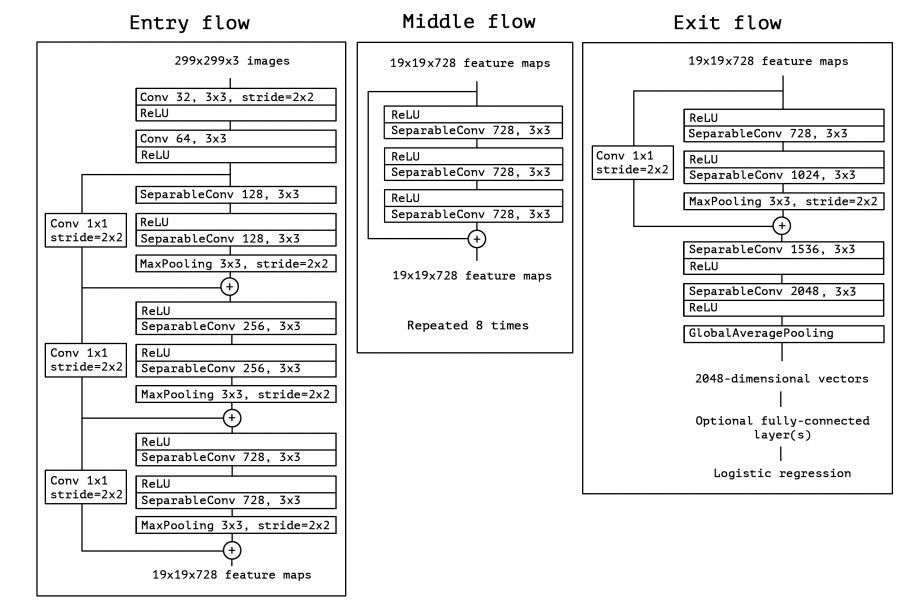
\includegraphics[width=0.7\textwidth]{xception/xception_architecture.jpg}
  \end{center}
  \caption{Xception Architecture}\label{f:xception_architecture}
\end{figure}

\subsubsection{Implementation}

To classify various brain tumour images, we will be proposing the Xception CNN architecture that is pre-trained on the \cite{ImageNet} dataset. By leveraging the pre-trained model, it allows extraction of lower-level data characteristics like edges and textures. This strategic approach significantly reduces the time and effort required for feature engineering while enhancing efficiency and accuracy in classification \cite{Pre-trainedModel}. To suit our usage, we modify the model by excluding the top output layer and then use the entire network as a fixed feature extractor for the new dataset, subsequently providing the input shape with $224\times224$ resized input image and with three channels. The enhancement of the input images is preprocessed during the Data Preprocessing phase.

To tailor the model to classify our tasks, we have strategically removed the last three layers. Additionally, we have added new layers to the model which include Global Average Pooling Layer, Dropout Layer, and Dense Layer with Softmax Activation. This modification replaces the fully connected layers by averaging each feature map to a single value, reducing the number of parameters and mitigating overfitting, while preserving spatial information more effectively. The dropout layer helps to prevent overfitting by randomly setting a fraction of the input units to zero during training, encouraging the model to learn more robust features that generalize better to new data. The final layer adds a dense layer that caters to our specific use case. In our dataset distribution, we learned that there are four different categories of images, hence implementing four neurons. Softmax and L2 regularization are used to output probabilities for each class and avoid overfitting by penalizing large weights.

Compilation of the model consists of Rectified-Adam (RAdam) Optimizer and categorical cross-entropy loss function. The RAdam plays a critical role in training the model, a new variant of the classic Adam optimizer that provides an automatic, dynamic adjustment to the adaptive learning rate regarding the effects of variance and momentum during training \cite{9259870}. Categorical cross-entropy is often used in multi-class classification, measuring the difference between the estimated probability and our desired outcome.

Execution on training the model incorporated several strategies to optimize performance and prevent overfitting. The use of \textit{ReduceLROnPlateau} callback monitors the validation loss and reduces the learning rate when improvement in the metric plateaus. Additionally, \textit{ModelCheckpoint} callback saves the model with the best validation loss during training, ensuring the retention of the most effective model. Employing \textit{EarlyStopping} callback ends the training process to avoid overfitting when the validation loss does not improve over a specified patience period. This approach is critical as it prevents the model from starting to learn noise from the training data, thus maintaining its generalization capabilities.


\subsubsection{Fine-Tuning}

Optuna, a hyperparameter optimization framework, was implemented to fine-tune the Xception model for image classification. The process begins with the preparation of the data, including initializing image generators for both training and validation datasets. These generators apply data augmentation techniques. Next, providing the suggested trial range of uniform \textit{dropout\_rate} and log-uniform \textit{learning\_rate}. These hyperparameters are critical as they control the regularization and the step size for the optimizer, respectively.

By running the optimization process, Optuna systematically explores different sets of hyperparameters across multiple trials. Specifically, ten trials are conducted, each with a different combination of hyperparameters. After the optimization process is complete, the best trial's results, including the optimal hyperparameters, are printed. 

Optuna significantly aids in fine-tuning the model by automating the hyperparameter tuning process. This automation saves time and effort compared to manual tuning. The result is a more robust and well-performing model, as Optuna helps to identify the best hyperparameters that leads to the lowest validation loss, thereby enhancing the overall performance on the image classification task.

\subsubsection{Results and Evaluation}


\begin{figure}[H]
    \centering
    \begin{subfigure}[b]{0.2\textwidth}
      \centering
      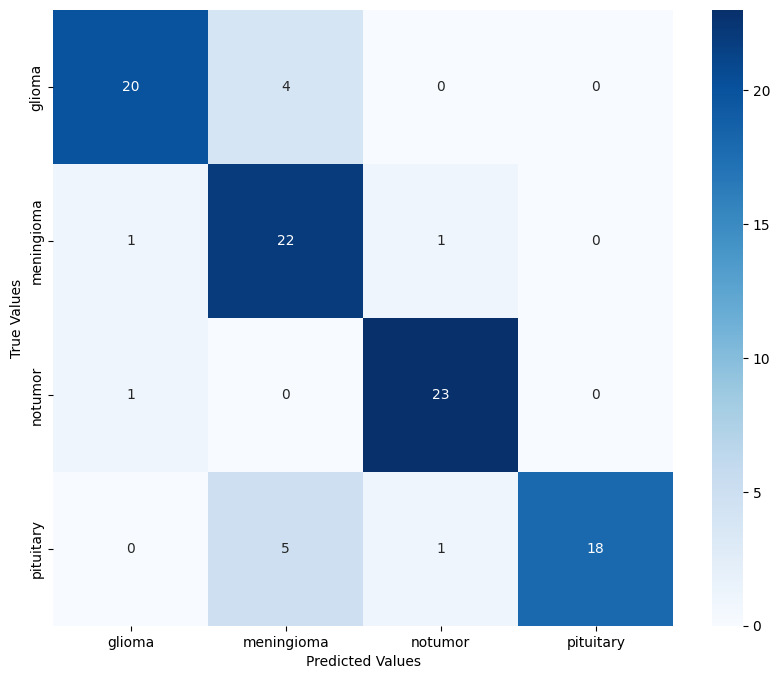
\includegraphics[width=\textwidth]{xception/evaluation/nt_cm1.png}
      \caption{Confusion Matrix}
      \label{fig:xception_nt_cm1}
    \end{subfigure}
    \hfill
    \begin{subfigure}[b]{0.2\textwidth}
      \centering
      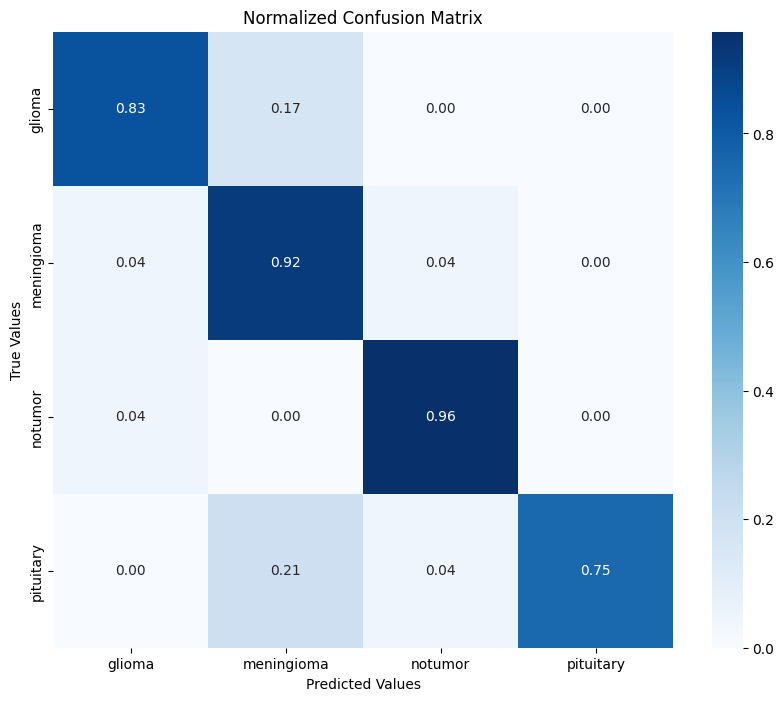
\includegraphics[width=\textwidth]{xception/evaluation/nt_cm2.png}
      \caption{Normalized Confusion Matrix}
      \label{fig:xception_nt_cm2}
    \end{subfigure}
    \hfill
    \begin{subfigure}[b]{0.25\textwidth}
      \centering
      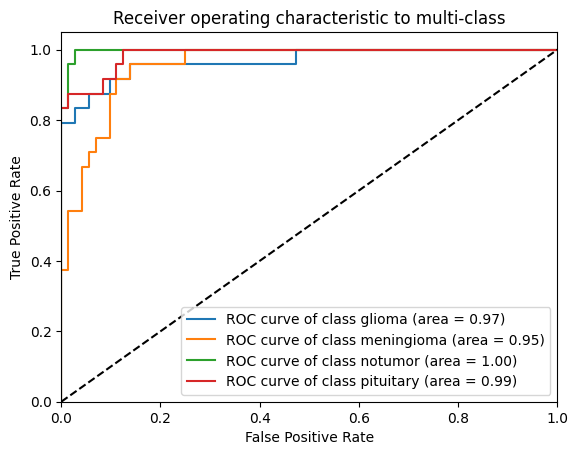
\includegraphics[width=\textwidth]{xception/evaluation/nt_ROC.png}
      \caption{ROC Curve}
      \label{fig:xception_nt_roc}
    \end{subfigure}
    \hfill
    \begin{subfigure}[b]{0.25\textwidth}
      \centering
      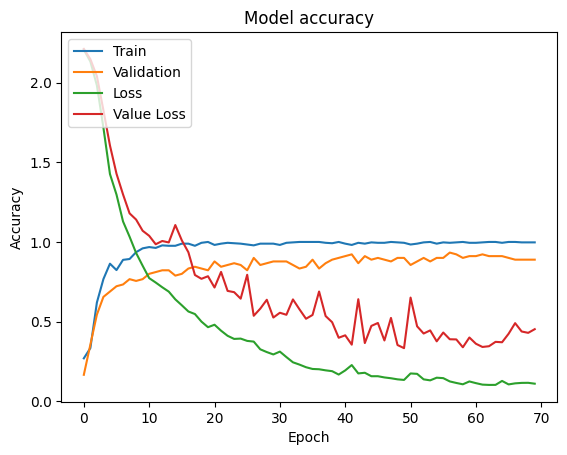
\includegraphics[width=\textwidth]{xception/evaluation/nt_learning_curve.png}
      \caption{Learning Curve}
      \label{fig:xception_nt_learning_curve}
    \end{subfigure}
    \caption{Confusion Matrix, Normalized Confusion Matrix, ROC Curve, and Learning Curve for Brain tumour Segmentation (Not-Tuned)}
    \label{fig:xception_nt_evaluation}
  \end{figure}
  
  \begin{figure}[H]
    \centering
    \begin{subfigure}[b]{0.2\textwidth}
      \centering
      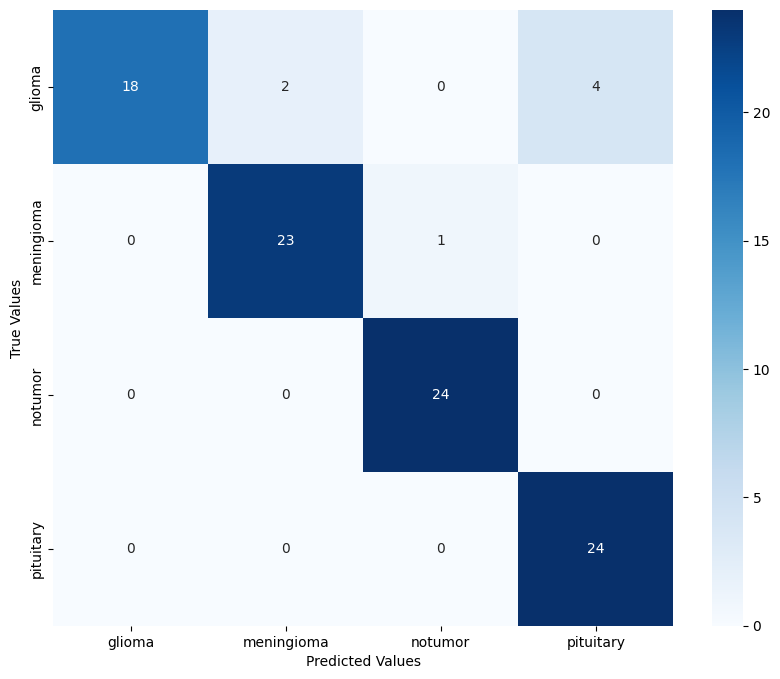
\includegraphics[width=\textwidth]{xception/evaluation/t_cm1.png}
      \caption{Confusion Matrix}
      \label{fig:xception_t_cm1}
    \end{subfigure}
    \hfill
    \begin{subfigure}[b]{0.2\textwidth}
      \centering
      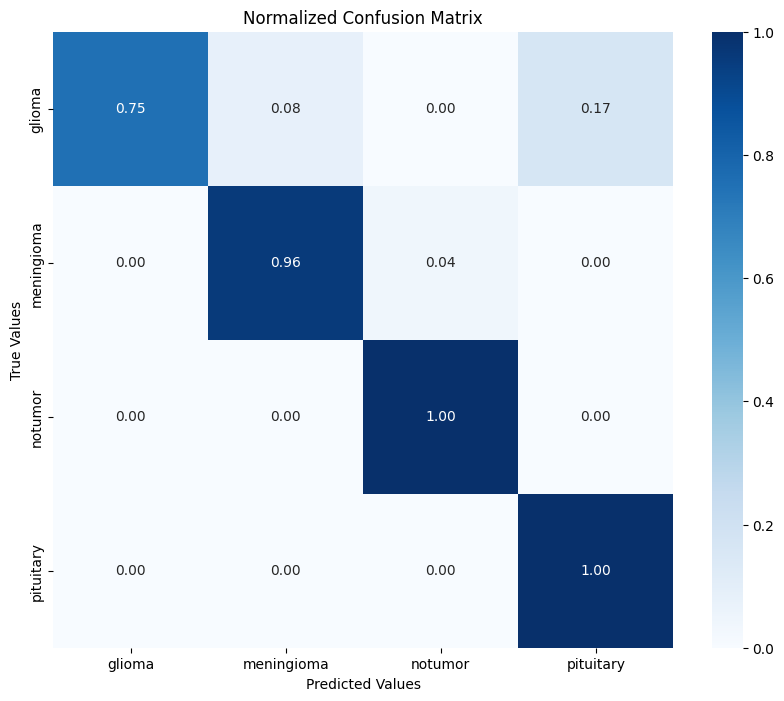
\includegraphics[width=\textwidth]{xception/evaluation/t_cm2.png}
      \caption{Normalized Confusion Matrix}
      \label{fig:xception_t_cm2}
    \end{subfigure}
    \hfill
    \begin{subfigure}[b]{0.25\textwidth}
      \centering
      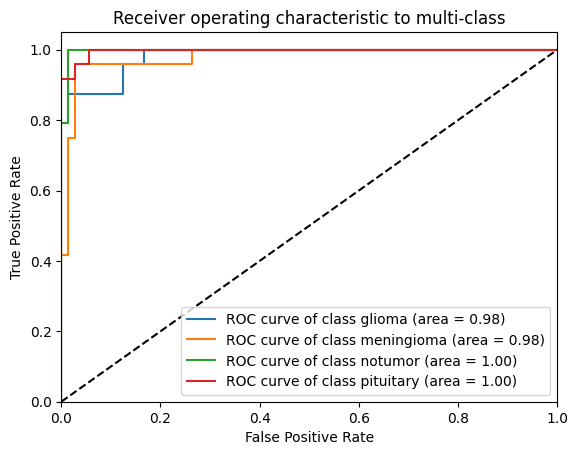
\includegraphics[width=\textwidth]{xception/evaluation/t_ROC.png}
      \caption{ROC Curve}
      \label{fig:xception_t_roc}
    \end{subfigure}
    \hfill
    \begin{subfigure}[b]{0.25\textwidth}
      \centering
      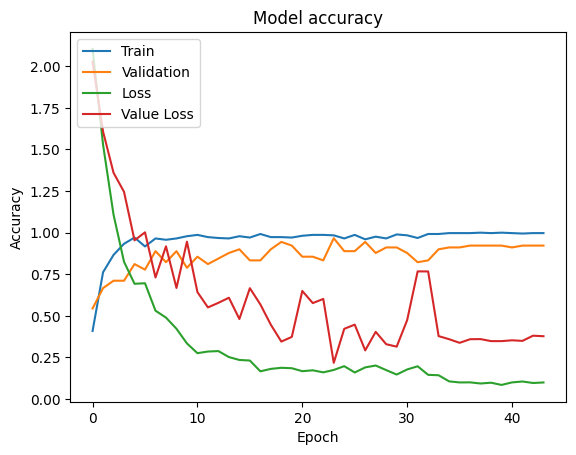
\includegraphics[width=\textwidth]{xception/evaluation/t_learning_curve.png}
      \caption{Learning Curve}
      \label{fig:xception_t_learning_curve}
    \end{subfigure}
    \caption{Confusion Matrix, Normalized Confusion Matrix, ROC Curve, and Learning Curve for Brain tumour Segmentation (Tuned)}
    \label{fig:xception_t_evaluation}
  \end{figure}
  
  \begin{table}[ht]
  \centering
  \begin{tabular}{cc}
      \begin{minipage}{.6\linewidth}
          \centering
          \begin{subtable}[t]{\linewidth}
              \centering
              \begin{tabular}{|l|c|c|c|c|}
                  \hline 
                  \textbf{Class} & \textbf{Precision} & \textbf{Recall} & \textbf{F1-Score} & \textbf{Support} \\ 
                  \hline 
                  meningioma & 0.71 & 0.83 & 0.77 & 24 \\ 
                  \hline
                  pituitary  & 1.00 & 0.79 & 0.88 & 24 \\ 
                  \hline
                  glioma     & 1.00 & 0.83 & 0.91 & 24 \\ 
                  \hline
                  notumour    & 0.83 & 1.00 & 0.91 & 24 \\ 
                  \hline
                  micro avg  & 0.86 & 0.86 & 0.86 & 96 \\ 
                  \hline
                  macro avg  & 0.89 & 0.86 & 0.87 & 96 \\ 
                  \hline
                  weighted avg & 0.89 & 0.86 & 0.87 & 96 \\ 
                  \hline
                  samples avg & 0.86 & 0.86 & 0.86 & 96 \\ 
                  \hline
              \end{tabular}
              \caption{Classification Report for Brain tumour Segmentation (Not-Tuned)} 
              \label{tab:xception_nt_classification_report}
          \end{subtable}
      \end{minipage} &
      \begin{minipage}{.35\linewidth}
          \centering
          \begin{subtable}[t]{\linewidth}
              \centering
              \begin{tabular}{|c|c|}
                  \hline 
                  \textbf{Metric} & \textbf{Value} \\ 
                  \hline
                  DSC & 0.8669 \\ 
                  \hline
                  Sensitivity & 0.8646 \\ 
                  \hline
                  Specificity & 0.9549 \\ 
                  \hline
                  Accuracy & 0.8646 \\ 
                  \hline
              \end{tabular}
              \caption{Additional Metrics for Brain tumour Segmentation (Not-Tuned)} 
              \label{tab:xception_nt_additional_metrics}
          \end{subtable}
      \end{minipage}
  \end{tabular}
  \caption{Classification Report and Additional Metrics for Brain tumour Segmentation using Xception (Not-Tuned)}
  \label{tab:combined_xception_nt_metrics}
  \end{table}
  
  \begin{table}[ht]
    \centering
    \begin{tabular}{cc}
        \begin{minipage}{.6\linewidth}
            \centering
            \begin{subtable}[t]{\linewidth}
                \centering
                \begin{tabular}{|l|c|c|c|c|}
                    \hline 
                    \textbf{Class} & \textbf{Precision} & \textbf{Recall} & \textbf{F1-Score} & \textbf{Support} \\ 
                    \hline 
                    meningioma & 0.92 & 0.96 & 0.94 & 24 \\ 
                    \hline
                    pituitary  & 0.86 & 1.00 & 0.92 & 24 \\ 
                    \hline
                    glioma     & 1.00 & 0.75 & 0.86 & 24 \\ 
                    \hline
                    notumour    & 0.96 & 1.00 & 0.98 & 24 \\ 
                    \hline
                    micro avg  & 0.93 & 0.93 & 0.93 & 96 \\ 
                    \hline
                    macro avg  & 0.93 & 0.93 & 0.92 & 96 \\ 
                    \hline
                    weighted avg & 0.93 & 0.93 & 0.92 & 96 \\ 
                    \hline
                    samples avg & 0.93 & 0.93 & 0.93 & 96 \\ 
                    \hline
                \end{tabular}
                \caption{Classification Report for Brain tumour Segmentation (Tuned)} 
                \label{tab:xception_t_classification_report}
            \end{subtable}
        \end{minipage} &
        \begin{minipage}{.35\linewidth}
            \centering
            \begin{subtable}[t]{\linewidth}
                \centering
                \begin{tabular}{|c|c|}
                    \hline 
                    \textbf{Metric} & \textbf{Value} \\ 
                    \hline
                    DSC & 0.9247 \\ 
                    \hline
                    Sensitivity & 0.9271 \\ 
                    \hline
                    Specificity & 0.97570 \\ 
                    \hline
                    Accuracy & 0.9271 \\ 
                    \hline
                \end{tabular}
                \caption{Additional Metrics for Brain tumour Segmentation (Tuned)} 
                \label{tab:xception_t_additional_metrics}
            \end{subtable}
        \end{minipage}
    \end{tabular}
    \caption{Classification Report and Additional Metrics for Brain tumour Segmentation using Xception (Tuned)}
    \label{tab:combined_xception_t_metrics}
    \end{table}


Figures \ref{fig:xception_nt_evaluation}, \ref{fig:xception_t_evaluation} and Tables \ref{tab:combined_xception_nt_metrics}, \ref{tab:combined_xception_t_metrics}, provide a detailed view of the model's before and after performance across the four brain tumour classes: meningioma, pituitary, glioma, and no tumour. Prior to the Optuna hyperparameter optimization, the model's elapsed epoch, \textit{dropout\_rate}, and \textit{learning\_rate} were 70, 0.2, and 0.0001, respectively. Upon optimization, the model's elapsed epoch, \textit{dropout\_rate}, and \textit{learning\_rate} were 44, 0.32072197395702773, and 0.0006410837916333897, respectively. Both had \textit{batch\_size} of 10 and optimizer parameters ($\beta_1$ of $0.9$, $\beta_2$ of $0.999$, and $\epsilon$ of $1 \times 10^{-8}$).

The confusion matrices in Figures \ref{fig:xception_t_cm1} and \ref{fig:xception_t_cm2} showcase strong classification results, indicating high precision for no tumour and pituitary classes with 1.00 accuracy while meningioma with 0.96 accuracy. Although glioma demonstrates slightly lower accuracy, the observations highlight the robustness of the model for most classes. 
The ROC (Receiver Operating Characteristics) curve in Figure \ref{fig:xception_t_roc} indicates excellent model performance with the area under the curve (AUC) values being 0.98 for both glioma and meningioma, and a perfect 1.00 for no tumour and pituitary. These results reflect the model's high discriminative ability across all classes.
The learning curve in Figure \ref{fig:xception_t_learning_curve} illustrates the model's accuracy and loss over 44 epochs, showing rapid initial improvements in both training and validation accuracy within the first few epochs, subsequently stabilizing throughout. The losses for both training and validation converge towards a stable performance, even though with minor fluctuations. Overall, indicating the model is learning effectively and moving towards a stable performance. 
The Table \ref{tab:xception_t_classification_report} shows high performance, with precision, recall and F1-scores across all classes, with a notable F1-score of 0.98 for the class of no tumour. The no tumour and meningioma classes exhibit particularly high metrics, reflecting the model's outstanding accuracy. Overall micro, macro and weighted averages all stand at 0.92 reflecting consistent and reliable performance. 
The Table \ref{tab:xception_t_additional_metrics} depicts the model's impressive performance metrics with a Dice Similarity Coefficient (DSC) of 0.9247, indicating excellent overlap between the predicted and actual tumour regions. The sensitivity and accuracy are both 0.9271, reflecting the model's high ability to correctly identify tumour cases. Additionally, the Specificity of 0.9757 showcases the model's strong performance in correctly identifying no tumour cases.


\subsubsection{K-Folds Cross-Validation}

\begin{figure}[H]
  \begin{center}
    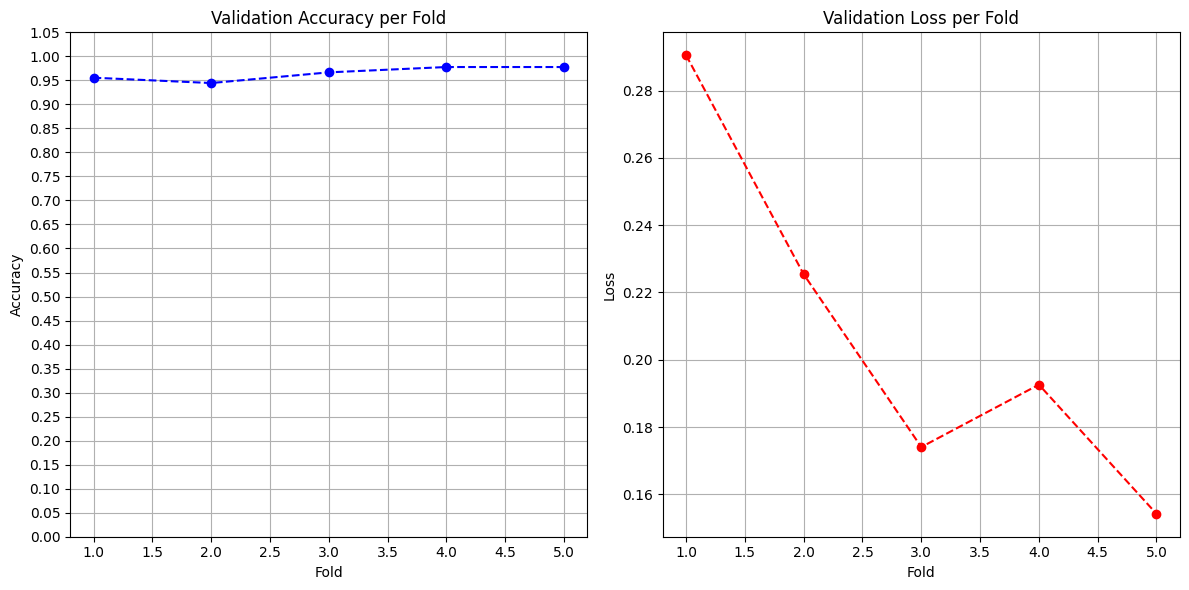
\includegraphics[width=0.7\textwidth]{xception/evaluation/t_kfolds.png}
  \end{center}
  \caption{K-Folds Cross-Validation for Brain tumour Segmentation (Tuned)}\label{f:xception_kfolds}
\end{figure}

To evaluate the model's performance on different subsets of the dataset, K-Folds cross-validation was employed. This method involves splitting the dataset into $k$ equal segments, known as folds. The model is trained on $k-1$ of these segments and tested on the remaining one. This process is repeated $k$ times, with each segment used as the test set once. The overall validation accuracy and loss, averaged over all folds, provide a thorough evaluation of the model's performance and its ability to generalize.

Tables \ref{tab:xception_kfolds_parameters} and \ref{tab:xception_kfolds_conditions} show the setup parameter configuration and the results from the K-Folds cross-validation. Execution of 5 folds, 90 epochs and a batch size of 10 aims to thoroughly assess the model's performance. The evaluation of the results indicated a robust performance, with an average validation accuracy of 0.9644 and an average validation loss of 0.2073. The consistency of the model's performance was further confirmed by the standard deviations, which were 0.0130 for validation accuracy and 0.0477 for validation loss. These metrics collectively highlight the model's reliability and generalizability across different subsets of the data.

\begin{table}[H]
\centering
\caption{K-Folds Cross-Validation Testing Conditions (Tuned)}\label{tab:xception_kfolds_conditions}
\begin{tabular}{cc}
    \begin{minipage}{.45\linewidth}
        \centering
        \begin{subtable}[t]{\linewidth}
            \centering
            \begin{tabular}{|l|c|}
                \hline
                \textbf{Parameter} & \textbf{Value} \\
                \hline
                Number of Folds ($k$) & 5 \\
                \hline
                Epochs & 90 \\
                \hline
                Batch Size & 10 \\
                \hline
            \end{tabular}
            \caption{Training Parameters}
            \label{tab:xception_kfolds_parameters}
        \end{subtable}
    \end{minipage} &
    \begin{minipage}{.45\linewidth}
        \centering
        \begin{subtable}[t]{\linewidth}
            \centering
            \begin{tabular}{|l|c|}
                \hline
                \textbf{Metric} & \textbf{Value} \\
                \hline
                Average Validation Accuracy & 0.9644 \\
                \hline
                Average Validation Loss & 0.2073 \\
                \hline
                Validation Accuracy Std. Dev. & 0.0130 \\
                \hline
                Validation Loss Std. Dev. & 0.0477 \\
                \hline
            \end{tabular}
            \caption{Evaluation Metrics}
            \label{tab:xception_kfolds_metrics}
        \end{subtable}
    \end{minipage}
\end{tabular}
\end{table}



\subsubsection{Conclusion}

Implementing the Xception model for brain tumour classification demonstrates significant potential in accurately identifying various tumour types. By leveraging depthwise separable convolutions, the Xception architecture enhances computational efficiency and performance. The model was fine-tuned using Optuna for optimal hyperparameters, leading to improved accuracy and reduced overfitting. The K-Folds cross-validation method confirmed the model's robustness, with high average validation accuracy and low standard deviation, indicating consistent performance. These results underscore the model's capability to generalize well across different subsets of the dataset, making it a reliable tool for medical image classification tasks.



